\chapter{Balanced cycle separators in planar graphs}

Let $G$ be a planar triangulation and let $w: F \to \mathbb{R}^+$ be face weight such that $\sum w = 1$ and $w(f) \leq 1/4$ for each face $f$. We would like to find a cycle $C$ in $G$ with property:
$$
\sum_{f \in Int(C)} w(f) \leq 3/4\qquad and \qquad \sum_{f\in Ext(C)} w(f) \leq 3/4
$$
where $Int(C)$ and $Ext(C)$ are interior and exterior faces with respect to the cycle $C$.

\medskip
\noindent Steps of the algorithm are:
\begin{enumerate}
\item Let $T$ be a tree with $\Delta(T) \leq 3$ and let $w: V(T) \to \mathbb{R}^+$ be vertex weight function with $\sum w = 1$ such that $w(v) \leq 1/4$ for each vertex $v$. Then there exist an edge $e$ such that $T - e = T_1 \cup T_2$ and $w(T_1) \leq 3/4$ and $w(T_2) \leq 3/4$. \\
Write function \verb`tree_weight_decomposition(T, w)` which finds such an edge. See hint in the code below for how to do this efficiently!

\item Choose a cycle $C_\infty$ to be the infinite cycle (outer face) and use modified BFS algorithm to find a BFS tree from $C_\infty$ and to determine distance $dist(v)$ from $C_\infty$ for each vertex $v \in V(G)$.

\item Find dual tree $T^*$ of the BFS tree $T$. Vertices of $T^*$ are faces of $G$ and two faces are connected if they are adjacent and the edge between them is not in $T$.

\item Use algorithm from Step 1 to find edge $e^* = (f, g)$ in $T^*$.

\item Find edge $e$ in $G$ which is common edge of faces $f$ and $g$. Then there is a cycle in $T \cup e$. This cycle $C$ is a solution of the algorithm.
\end{enumerate}

\section{Implemetation}

\subsection*{Auxilliary functions}

\begin{sageCell}
    def BFS(G, S):
    import queue

    prev = {}
    dist = {}
    q = queue.Queue()
    for s in S:
        prev[s] = None
        dist[s] = 0
        q.put(s)
    while not q.empty():
        v = q.get()
        for u in G.neighbors(v):
            if u not in prev:
                prev[u] = v
                dist[u] = dist[v] + 1
                q.put(u)
    return prev, dist

def face_edges_to_tuple(F):
    return tuple([u for (u, v) in F])

def tuple_to_face_edges(T):
    """Convert a tuple (a1, a2, ..., ak) representing a face to
    a list of 'edges' [(a1, a2), (a2, a3), ..., (ak, a1)] """
    f = []
    for i in range(len(T)):
        f.append((T[i], T[(i + 1) % len(T)]))
    return f

def face(G):
    """Find one face (sequence of vertices on it); call after embedding is set
    """
    return [a for (a, b) in G.faces()[0]]
\end{sageCell}

\begin{sageCell}
    G = Graph('K{mkXOXC[_{J')  # Planar triangulation
    G.is_planar(set_embedding=True, set_pos=True)  # find planar embedding
    Tr = face(G)  # take the first triangle to be our "initial" triangle
    G.plot(edge_colors={"red": tuple_to_face_edges(Tr)})
\end{sageCell}
\begin{outImage}
   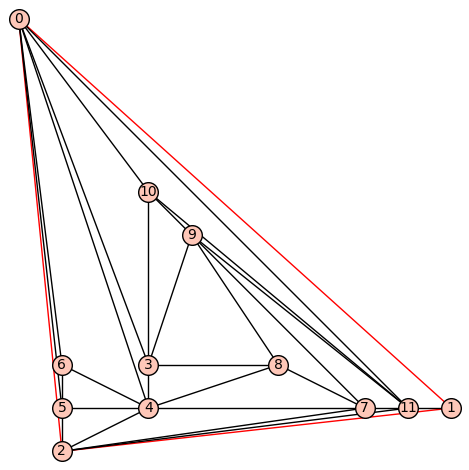
\includegraphics[width=0.6\textwidth]{Images/BalancedSeparators/initial_triangle.png}
\end{outImage}


\subsection*{Step 1}

\begin{sageCell}
def tree_weight_decomposition(T, w):
    """
    Arguments
    T tree, Delta(T) <= 3
    w weights, w: V(T) -> R+, sum w(v) = 1, w(v) <= 1/4

    Result is edge e = (u, v) such that G = T1 + e + T2 and
    w(T1) <= 3/4, w(T2) <= 3/4
    Algorithm should be linear in the number of vertices (edges)
    """
    # See:
    # https://planarity.org/Klein_rooted_forests_and_trees.pdf
    # Lemma 1.3.2
    # Or:
    # Let eweights[(u, v)] be a weight of the component of T - (u, v) containing u
    # Calculate eweights[(u, v)] for each (directed) edge (u, v). You can do this recursively.
    # Find edge e = (u, v) for which difference abs(eweights[(u, v)] - ewighths[(v, u)]) is minimal and return e
    eweights = {}
    mindif = None
    e = None
    for u, v in T.edges(labels = False, sort=False):
        wuv = edge_weight_memo(eweights, T, w, (u, v))
        wvu = edge_weight_memo(eweights, T, w, (v, u))
        if mindif == None or abs(wuv - wvu) < mindif:
            mindif = abs(wuv - wvu)
            e = (u, v)
    return e

def edge_weight_memo(eweights, T, w, e):
    (u, v) = e
    if (u, v) in eweights:
        return eweights[(u, v)]
    else:
        weight = w[u]
        for x in T.neighbors(u):
            if x != v:
                weight += edge_weight_memo(eweights, T, w, (x, u))
        eweights[(u, v)] = weight
        return weight
\end{sageCell}

\section*{Step 2}

\begin{sageCell}
def BFS_graph(G, S):
    """
    G: triangulation,
    S: 'outer' face
    result is pair (T, dist) where is 'tree' from S together with edges of S
    and dist is distance map from S
    """
    prev, dist = BFS(G, S)
    edges = [(u, v) for (u, v) in prev.items() if v != None]
    edges.extend(tuple_to_face_edges(S))
    return Graph(edges), dist
\end{sageCell}

\begin{sageCell}
    BFS_graph(G, Tr)[0].plot()
\end{sageCell}

\begin{outImage}
   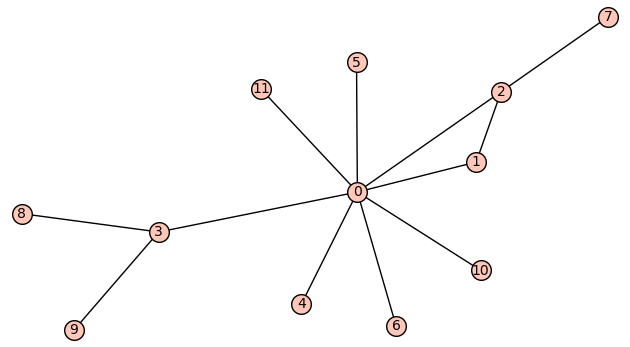
\includegraphics[width=0.6\textwidth]{Images/BalancedSeparators/bfs_tree.png}
\end{outImage}

\begin{sageCell}
    BFS_graph(G, Tr)[1]
\end{sageCell}

\begin{outCell}
    {0: 0, 1: 0, 2: 0, 3: 1, 4: 1, 5: 1, 6: 1, 10: 1, 11: 1, 7: 1, 8: 2, 9: 2}
\end{outCell}
Explanation: dictionary above gives the distances for each vertex from the outer triangle (4, 7, 8)

\section*{Step 3}

\begin{sageCell}
def dual_tree(G, BFSG):
    """Step 3 of the algorithm. Find dual tree. BFSG is the (first) result of the BFS_graph function above
    """
    efaces = G.faces()
    bfsedges = BFSG.edges(labels=False, sort=False)
    edgetoface = {}
    for ef in efaces:
        f = face_edges_to_tuple(ef)
        for u, v in ef:
            edgetoface[(u, v)] = f
    edges = []
    for u, v in G.edges(labels=False, sort=False):
        if (u, v) not in bfsedges and (v, u) not in bfsedges: # lin?
            edges.append((edgetoface[(v, u)], edgetoface[(u, v)]))
    return Graph(edges)
\end{sageCell}

\begin{sageCell}
    dual_tree(G, BFS_graph(G, Tr)[0])
\end{sageCell}
\begin{outImage}
    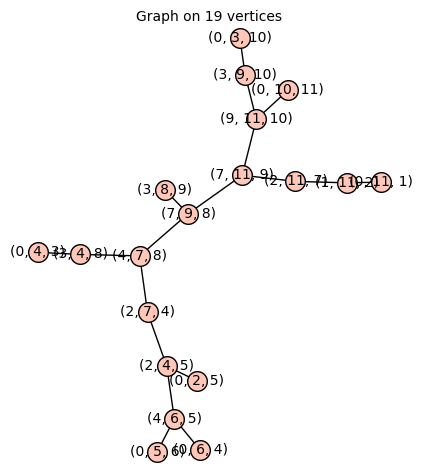
\includegraphics[width=0.6\textwidth]{Images/BalancedSeparators/dual_tree.png}
\end{outImage}
Explanation: Vertices of this graph are faces of the triangulation (except of outer face $(4, 7, 8)$). Two vertices (faces) are connected precisely when the faces are adjacent and the edge between the two faces is not in the BFSG.
For example, faces $(0, 3, 10)$ and $(10, 11, 0)$ are not connected since the edge between them $(0, 10)$ is in the BFSG (see image above), while there is an edge between $(0, 3, 10)$ and $(3, 0, 4)$ since the edge between them $(0, 3)$ is not in BFSG.

\section*{Put everything together}

\begin{sageCell}
def find_cycle_separator(G, S, w):
    BT, dist = BFS_graph(G, Tr)
    DT = dual_tree(G, BT)
    faces = DT.vertices(sort=False)
    finf = tuple(S)
    n = G.num_verts()
    wsum = sum(w.values())

    # Find edge in dual tree
    (fu, fv) = tree_weight_decomposition(DT, w)

    # Find edge in BFS tree
    e = [(u, v) for (u, v) in tuple_to_face_edges(fu) if (v, u) in tuple_to_face_edges(fv)][0]

    # Create cycle
    prev, _ = BFS(BT, [e[0]])
    C = [e[1]]
    while prev[C[-1]] != None:
        C.append(prev[C[-1]])

    return C # , dist, FC, len(faces)
\end{sageCell}
Plot solution:
\begin{sageCell}
    # make uniform weights
    w = dict([(face_edges_to_tuple(f), 1/len(G.faces())) for f in G.faces()])
    C = find_cycle_separator(G, Tr, w)
\end{sageCell}

\begin{sageCell}
    G.plot(edge_colors={"red": tuple_to_face_edges(C)})
\end{sageCell}
\begin{outImage}
    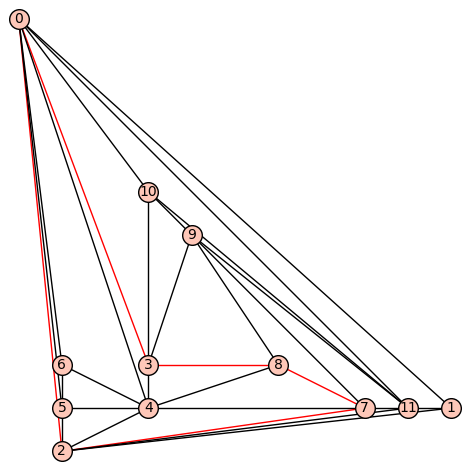
\includegraphics[width=0.6\textwidth]{Images/BalancedSeparators/cycle_separator.png}
\end{outImage}

\begin{sageCell}
    C
\end{sageCell}
\begin{outCell}
    [8, 3, 0, 2, 7]
\end{outCell}
Explanation; the number (since we use uniform weights) of triangles inside and outside red cycle is "balanced", i.e., $\leq 3/4$ of the total number of triangles.
